%!TEX root = cvičení NUM - kindle.tex
%
%  Cvičení z NUM
%
%  Created by Matěj Novotný on 2011-02-24.
%  Copyright (c) 2011 Matěj Novotný. All rights reserved.
%

%\documentclass[12pt]{article}
\usepackage[utf8]{inputenc}
\usepackage[czech]{babel}

%\usepackage{ifthen}

%\newboolean{kindle}

% kindle verze = true, A4 verze = false
%\setboolean{kindle}{false} 

\newcommand{\kindle}[2]{\ifthenelse{\boolean{kindle}}{#1}{#2}}

\kindle{\usepackage[top = 1.5cm, bottom=2cm, left=0.8cm, right=0.8cm, a5paper]{geometry}}
{
\usepackage[a4paper]{geometry}
\usepackage{fullpage}
}

\usepackage[pdftex]{graphicx}
\usepackage{ifpdf}
\usepackage[pdftex]{hyperref}
\hypersetup{
	pdftitle={Zapisky z cviceni NUM 2011},
	pdfauthor={Matej Novotny},
	pdfkeywords={FJFI, numericka matematika}
}

% matematika a symboly
\usepackage{amsmath}
\usepackage{amssymb}
\usepackage{amsthm}
\usepackage{latexsym}

\usepackage{graphicx}


\newtheorem{definition}{Definice}
\newtheorem{theorem}{Věta}
\newtheorem{lemma}{Lemma}
\newtheorem{example}{Příklad}
\newtheorem{note}{Poznámka}

\newcommand{\inte}[2]{\int\limits_0^1 #1\,\mathrm{d}#2}
\newcommand{\R}{\mathbb{R}}
\newcommand{\pa}{\partial}

\title{Zápisky z cvičení NUM 2011}
\author{Matěj Novotný}
\date{\today}

\setlength{\parindent}{0pt}

\begin{document}

	
	\maketitle
	\section{Diferenční vztahy pro náhrady derivací}
	
	\kindle{
		\thispagestyle{empty}
		\pagestyle{empty}
	}{}
	
	\begin{note}[Taylorův rozvoj]
		Nechť $g \in C^{(m)}$ na $\langle a,b \rangle;\ x\in (a,b);\ 0<h<min\{x-a,b-x\}$. Pak je
		\begin{equation} \label{diference}
			g(x+h)=\sum_{k=0}^{m-1} \frac{1}{k!} g^{(k)}(x) h^k +
			h^m\inte{\frac{1}{m!} s^{m-1} g^{(m)} (x+(1-s)h)}{s}
		\end{equation}
		Druhý sčítanec je Lagrangeův tvar zbytku.
	\end{note}
	
	\begin{definition}[Landaův symbol $O$]
		Nechť $f:H_0 \rightarrow \R$ je funkce definovaná na prstencovém okolí 0 ($H_0$).
		Řekneme, že $f$ se chová na $H_0$ jako $h^\alpha$ pro nějaké $\alpha \in \R$
		(značíme $f(x) = O(h^\alpha)$), právě když
		\begin{equation} \label{landau}
			(\exists K > 0)(\forall h \in H_0 - \{0\}) 
			\left( \left| \frac{f(h)}{h^\alpha}\right|  <K \right)	
		\end{equation}
		
	\end{definition}
	
	\begin{note}
		Chyba aproximace závisí na h.
	\end{note}
	
	\begin{theorem}
		Nechť $g \in C^{(2)}$ na $\langle a,b \rangle;\ x \in (a,b);\ 0 < h < \min\{x-a, b-x\}$. Pak
		\begin{align*}
			\frac{g(x+h) -g(x)}{h} &= g'(x) + O(h)\quad \text{(dopředná diference)}\\
			\frac{g(x) - g(x-h)}{h} &= g'(x) + O(h)\quad \text{(zpětná diference)}\\
		\end{align*}
	\end{theorem}
	
	\begin{proof}
		V Taylorově rozvoji \eqref{diference} použijeme $m=2$.
		$$ g(x+h) = g(x) h^0 + g'(x)h + h^2 \inte{\frac{1}{2!} s^1 g^{(2)}(x+(1-s)h)}{s}$$
		$$ \frac{g(x+h) - g(x)}{h} = g'(x) + h\inte{\frac{1}{2} s g^{(2)}(x+(1-s)h)}{s}$$
		Je poslední člen roven $O(h)$? $g \in C^{(2)}(\langle a, b\rangle) \implies g^{(2)}
		\in C(\langle a, b\rangle)$, tj. $g^{(2)}$ je spojitá na $\langle a, b\rangle \implies
		g^{(2)}$ je omezená na $\langle a, b\rangle \implies g^{(2)}(x) < K$ na
		$\langle a, b\rangle$.
		$$ \frac{1}{2} \inte{s g^{(2)}(x+(1-s)h)}{s} \leq \frac{1}{2}\inte{sK}{s} = 
		\frac{K}{2}\inte{s}{s} = \frac{K}{4}$$
		$$ \left| \frac{g(x+h) - g(x)}{h} - g'(x) \right|= h \left|\inte{\frac{1}{2} s g^{(2)}
		(x + (1 -s) h)}{s}\right| \leq h\frac{K}{4}$$
		$$ \frac{\left| \frac{g(x+h) - g(x)}{h} - g'(x) \right|}{|h|} \leq \frac{K}{4} \implies
		\frac{g(x+h) - g(x)}{h} - g'(x) = O(h)$$
		Druhý vzorec se dokáže úplně stejně až na znaménko $-$.
	\end{proof}
	
	\begin{theorem}
		Nechť $g \in C^{(3)} (\langle a,b \rangle);\ x \in (a,b);\ 0 < h < \min\{ x-a, b-x\}$.
		Pak
		$$ \frac{g(x+h) - g(x-h)}{2h} = g'(x) + O(h^2)$$
	\end{theorem}
	
	\begin{proof}
		$$ g(x \pm h) = g(x) \pm h g'(x) + h^2 \inte{\frac{1}{2} s g^{(2)}
		(x \pm (1-s) h)}{s}$$
		$$ g(x+h) - g(x-h) = g(x) + hg'(x) + \frac{h^2}{2} \inte{s g^{(2)} (x + (1-s) h)}{s} -$$
		$$ - ( g(x) - hg'(x) + \frac{h^2}{2} \inte{s g^{(2)} (x - (1-s) h)}{s}) =$$
		\begin{equation} \label{dk1}
			 = 2hg'(x) + \frac{h^2}{2} \inte{s \left[ g^{(2)} (x + (s-1)h) - g^{(2)}
			(x - (1-s)h) \right]}{s}
		\end{equation}
		$$ \left| \frac{g(x+h) - g(x-h)}{2h} - g'(x)\right| = \frac{h}{4} \left|
		\inte{\dots}{s}\right| \leq h \frac{K}{4} $$
		To znamená, že zbytek je $O(h)$. Použijeme Lagrangeovu větu o přírůstku funkce
		($\exists \xi:g(a) - g(b) = g'(\xi)(a -b)$):
		$$ \exists \xi= \xi(s,x,h);\ \xi \in (x- (1-s)h, s+(1-s)h) \subset \langle a,b \rangle$$
		$$ g^{(2)} (x+(1-s)h) - g^{(2)} (x-(1-s)h) = g^{(3)} (\xi) (x+(1-s)h - x +(1-s)h) =$$
		$$ = g^{(3)}(\xi) 2 (1-s) h$$
		Dosadíme do integrálu \eqref{dk1}:
		$$ \inte{s g^{(3)} (\xi) 2 (1-s)h}{s} = 2h \inte{g^{(3)} (\xi) s (1-s)}{s} $$
		$g^{(3)}$ je spojitá $\implies$ je omezená na $\langle a,b \rangle$
		$$ 2h \left| \inte{g^{(3)}(\xi) s(s-s)}{s} \right| \leq 2hK \left| \inte{s(s-s)}{s} \right|
		\leq Kh$$
		Po dosazení do \eqref{landau} dostávám tvrzení věty.
	\end{proof}
	
	\begin{note}
		Vynechávám domácí úkol a nějaké povídání k němu. \href{http://geraldine.fjfi.cvut.cz/~oberhuber/data/vyuka/num/dcv1.pdf}{Tady najdete zadání.}
	\end{note}
	
	\kindle{
	\section{Numerické řešení ODR s počáteční \\podmínkou}
	}{\section{Numerické řešení ODR s počáteční podmínkou}}
	
	Máme problém
	\begin{align*}
		y'(x) &= f(x,y(x)) \\
		y(x_0) &= y_0
	\end{align*}

	Snažíme se nalézt vztah tvaru
	$$ y(x_0 + h) \approx y(x_0) + \Delta y(x_0)$$
	Člen $y(x_0)$ označíme $y_0$.
	
	Máme teoretickou možnost použít Taylorova rozvoje
	$$ \Delta y_0 = y(x+h) - y(x_0) = hy'(x_0) + \frac{h^2}{2}y''(x_0) + \dotsb$$
	$$ y'(x_0) = f(x_0,y_0)$$
	$$ y''(x_0) = f'(x_0,y(x_0)) = \pa_x f(x_0,y_0) + \pa_y f(x_0,y_0)\cdot y'(x_0)=$$
	$$ = \pa_x f(x_0,y_0) + \pa_y f(x_0,y_0)\cdot f(x_0,y_0)$$
	$$ \Delta y_0 = h \cdot f(x_0,y_0) + \frac{h^2}{2}\left( \pa_x f(x_0,y_0) + \pa_y f(x_0,y_0)
	\cdot f(x_0,y_0) \right)$$
	Tato metoda má složité vzorce a špatnou stabilitu.
	
	\subsection{Runge-Kuttovy metody}
	
	Navrhujeme $\Delta y_0$ ve tvaru
	$$\Delta y_0 = p_1 k_1 (h) + p_2 k_2 (h) + \dots + p_n k_n (h)$$
	kde
	\vspace{-1ex}
	\begin{align*}
		k_1 (h) &= h f(x_0,y_0) \\
		k_2 (h) &= h f(x_0 + \alpha_2 h,y_0 + \beta_{21} k_1 (h)) \\
		k_3 (h) &= h f(x_0 + \alpha_3 h,y_0 + \beta_{31} k_1 (h) + \beta_{32} k_2 (h)) \\
		\vdots \\
		k_n (h) &= h f(x_0 + \alpha_n h,y_0 + \beta_{n1} k_1 (h) + \dots + \beta_{n,n-1}
		k_{n-1} (h))
	\end{align*}
	
	Sem Matěj doplní zápisky z druhého cvičení.
	
	\subsection{Mexsonova metoda}
	
	\begin{enumerate}
		\item \begin{align*}
			k_1 &= hf_0 \\
			k_2 &= hf\left(x_0 + \frac{h}{3},\ y_0 + \frac{k_1}{3} \right) \\
			k_3 &= hf\left(x_0 + \frac{h}{3},\ y_0 + \frac{k_1}{6} + \frac{k_2}{6} \right) \\
			k_4 &= hf\left(x_0 + \frac{h}{2},\ y_0 + \frac{k_1}{8} + \frac{3k_3}{8} \right) \\
			k_5 &= hf\left(x_0 + h,\ y_0 + \frac{k_1}{2} - \frac{3k_3}{2} + 2k_4 \right) \\
		\end{align*}
		\item Chyba:
			$$ e = \frac{1}{3} \left| \frac{k_1}{5} - \frac{9k_3}{10} + \frac{4k_4}{5} -
			\frac{k_5}{10}\right| $$
		\item Pokud $ e < \varepsilon,\ y(x_0 + h) = y(x_0) + \frac{1}{6}(k_1 + 4k_4 + k_5)$
		\item $$ h := h \frac{4}{5} \left( \frac{\varepsilon}{e}\right)^{\frac{4}{5}} $$
	\end{enumerate}
	
	Druhý úkol je taktéž na \href{http://geraldine.fjfi.cvut.cz/~oberhuber/data/vyuka/num/dcv2.pdf}{webu}.
	
	\begin{align*}
		-(p(x) y')' + q(x)y &= f(x) \text{ na } (a,b) \\
		y(a) &= \gamma_1 \\
		y(b) &= \gamma_2 \\
		y &= y(x)
	\end{align*}
	
	Zavedeme numerickou síť
	\begin{align*}
		\overline{\omega_h} &= \{ a + jh| j \in \widehat{m_0}\} \\
		\omega_h &= \{ a + jh| j \in \widehat{m-1}\}.
	\end{align*}
	
	$$ -(pu_{\overline{x}})_x + qu =f \text{ na } \omega_k;\ u_0 = \gamma_1,\ u_m = \gamma_2 $$
	$$ u_{\overline{x_i}} = \frac{u_{i+1} - u_i}{h} \quad \text{zpětná diference} $$
	
	Hledáme přesnost aproximace
	$$ \psi = L_h(P_h y ) - P_h(L_y).$$
	$P_h$ je projekce funkcí definovaných na $(a, b)$ do funkcí definovaných na síti $\overline{\omega_h}$.
	\begin{align*}
		\psi &= -(p(P_h y)_{\overline{x}})_x + qP_hy - f - P_h(-(py')' + qy - f) \\
		\psi_j &= -(p(P_h y)_{\overline{x}})_x - P_h(-(py')') \quad \rightarrow O(h)
	\end{align*}
	$$ - \frac{1}{h} \left( p_{i + \frac{1}{2}} \frac{u_{i+1} - u_i}{h} - p_{i - \frac{1}{2}}
	\frac{u_i - u_{i-1}}{h} \right)  + qu_i = f_i \text{ na } \omega_h$$
	$$ u_0 = \gamma_1;\ u_m = \gamma_2 $$
	$$ p_{i \pm \frac{1}{2}} = p\left(a + \left(i \pm \frac{1}{2}\right)h \right) \quad
	\rightarrow O(h^2)$$
	\begin{enumerate}
		\item ~\\ 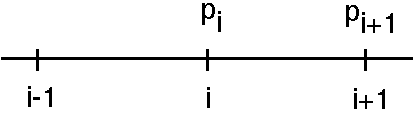
\includegraphics{mexson1.pdf}
			$$ (pu_{\overline{x}})_x = \frac{(pu_{\overline{x}})_{i+1} - (pu_{\overline{x}})_i}
			{h} = \frac{1}{h^2} (p_{i+1}(u_{i+1} - u_i) - p_i(u_i - u_{i-1})) $$
		\item ~\\ 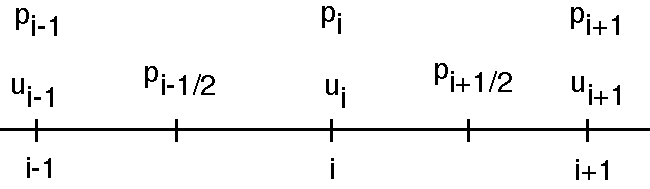
\includegraphics{mexson2.pdf}
			$$ (pu')' \approx \frac{pu'|_{i + \frac{1}{2}} - pu'|_{i - \frac{1}{2}}}{h} =
			\frac{1}{h^2}(p_{i + \frac{1}{2}}(y_{i+1} - y_i) - p_{i - \frac{1}{2}}(y_i - y_{i-1}))$$
			\begin{align*}
				p_{i + \frac{1}{2}} &= \frac{1}{2}(p_i + p_{i+1}) \\
				p_{i - \frac{1}{2}} &= \frac{1}{2}(p_i + p_{i-1})
			\end{align*}
	\end{enumerate}
	
\end{document}
